% ============================================================
% MineWorld-Enhancement: 面向实时交互世界模型的帧级投机解码
% 顶刊风格（ICML/NeurIPS 双栏格式，可独立编译，无外部依赖）
% ============================================================
\documentclass[10pt, twocolumn]{article}

\usepackage[T1]{fontenc}
\usepackage[utf8]{inputenc}
\usepackage{microtype}
\usepackage{amsmath,amssymb,amsfonts}
\usepackage{booktabs}
\usepackage{graphicx}
\usepackage{xcolor}
\usepackage{tikz}
\usetikzlibrary{arrows.meta, positioning, fit, backgrounds}
\usepackage{multirow}
\usepackage{enumitem}
\usepackage{hyperref}
\usepackage{float}
\usepackage{caption}
\usepackage{subcaption}
\usepackage{balance}

\definecolor{linkcolor}{RGB}{0,102,204}
\hypersetup{
  colorlinks=true,
  linkcolor=linkcolor,
  citecolor=linkcolor,
  urlcolor=linkcolor,
  pdfauthor={Anonymous},
  pdftitle={Frame-Level Speculative Decoding for Real-Time Interactive World Models}
}

% ---------- 页边距（仿顶刊） ----------
\usepackage[top=1in, bottom=1in, left=0.9in, right=0.9in]{geometry}

% ---------- 标题区 ----------
\title{\bf Frame-Level Speculative Decoding for Real-Time Interactive World Models: A Systematic Study of Speed--Quality Trade-offs}

\author{
  Anonymous Author(s)\\
  \texttt{anonymous@example.com}
}
\date{}

\begin{document}
\maketitle

\begin{abstract}
Real-time interactive world models must autoregressively generate future video frames from visual observations and player actions, where per-frame latency directly bounds interactive fidelity. Diagonal decoding reduces the 336 sequential forward passes of a $14\times24$ VQ token grid to roughly 60 passes, yet this remains the dominant runtime bottleneck. In this work, we study \emph{frame-level speculative decoding}---a lightweight draft model proposes an entire frame (336 tokens) in a single forward pass, and an action-verification gate decides whether to accept the draft frame or fall back to full decoding. Through a systematic engineering study, we raise speculative decoding from a non-functional state ($0.42$ FPS) to parity with the diagonal-decoding baseline. On a paired 197-clip evaluation, frame-level speculation achieves a mean speedup of $1.012\times$ (median $1.024\times$) over the baseline, at a mean PSNR cost of $1.5$ dB. Crucially, we precisely characterize \emph{where the time goes}: each diagonal step costs $\sim$9 ms of GPU kernel time \emph{regardless of the number of tokens decoded in that step}, revealing a fixed per-step overhead (small-batch attention kernel inefficiency) as the true bottleneck, rather than draft latency or CPU--GPU synchronization. We identify two architectural obstacles that bound speculative gains: (i) \emph{verification lag}---the main stream redundantly decodes frames that the draft already proposed, and (ii) \emph{the fixed per-step decode cost}---which leaves no GPU idle window in which to hide draft latency. We further introduce \emph{tolerant action verification}, which accepts near-miss camera actions within a configurable tolerance, raising the acceptance rate substantially at negligible additional quality cost. Our findings provide actionable guidance for accelerating autoregressive world models and clarify when speculative decoding can---and cannot---pay off under single-GPU constraints.
\end{abstract}

\section{Introduction}
\label{sec:intro}

World models that simulate interactive environments in real time~\cite{mineworld} are a cornerstone of embodied AI. A visual--action autoregressive transformer ingests past frames and player actions, and predicts the evolution of the game world frame by frame. Because each frame is a $14\times24=336$ grid of VQ tokens, naive row-major autoregressive generation requires 336 sequential transformer forward passes per frame---far too slow for real-time interaction.

Diagonal decoding~\cite{mineworld} exploits the 2-D spatial dependency structure of the token grid: tokens on the same anti-diagonal are mutually independent and can be predicted in parallel, reducing the number of sequential steps from 336 to roughly 60. On an RTX 3090, this yields approximately $2.77$ FPS for a 300M-parameter model. However, each of these $\sim$60 passes is a full forward through the entire network, and---as we show in Section~\ref{sec:obstacles}---the wall-clock cost of each pass is dominated by host-side orchestration rather than the GPU kernel itself.

Speculative decoding~\cite{leviathan2023fast,chen2023accelerating} accelerates autoregressive generation by using a small draft model to propose candidate tokens that a large target model verifies in parallel. The classical formulation targets \emph{token-level} speculation over 1-D sequences. Transferring this idea to \emph{frame-level} speculation over 2-D token grids raises two questions: (i) can a draft model propose an entire frame (all 336 tokens) in one forward pass, and (ii) can the acceptance mechanism avoid re-decoding the frame that the draft has already proposed?

In this paper, we systematically study frame-level speculative decoding for interactive world models. Our contributions are:

\begin{itemize}[leftmargin=1.4em, itemsep=1pt, topsep=2pt]
  \item We present a frame-level speculative decoding framework for diagonal-decoded world models, comprising a depth-aware draft model (13.9M parameters) that proposes a full frame in a single forward pass, and an action-verification gate that accepts or rejects the proposal.
  \item We identify and quantify two architectural obstacles---\emph{verification lag} and the \emph{fixed per-step decode cost}---that prevent naive speculation from surpassing the baseline, and provide a precise GPU-time breakdown that explains \emph{why}: each diagonal step costs $\sim$9 ms of GPU kernel time independent of how many tokens it decodes.
  \item We introduce \emph{tolerant action verification}, which accepts camera actions within a configurable bin tolerance, substantially raising the acceptance rate with a small, controllable quality cost.
  \item Through a systematic engineering study, we raise speculative decoding from a non-functional state ($0.42$ FPS) to parity with the diagonal-decoding baseline, and report a speed--quality Pareto frontier. On a paired 197-clip evaluation, we show that speculation reaches a mean speedup of $1.012\times$ over the baseline, and characterize when it helps and when it does not.
\end{itemize}

\section{Background and Setup}
\label{sec:background}

\subsection{MineWorld World Model}
MineWorld~\cite{mineworld} is a visual--action autoregressive world model for the Minecraft environment. Given a set of conditioning frames and a sequence of player actions (keyboard keys and camera deltas), the model predicts future frames. Each frame is tokenized by a VQ-VAE into a $14\times24$ grid of 336 discrete tokens, and the transformer predicts these tokens autoregressively.

\subsection{Diagonal Decoding}
Because row-major generation requires 336 sequential steps, MineWorld adopts diagonal decoding: tokens along the same anti-diagonal $(i,j)$ with constant $i+j$ are mutually independent and are predicted jointly in one forward pass. With a windowed schedule (window size 2), a $14\times24$ grid is generated in approximately 60 steps. This is the baseline we compare against.

\subsection{Speculative Decoding}
Speculative decoding~\cite{leviathan2023fast,chen2023accelerating} accelerates a large target model $M$ with a small draft model $D$. The draft proposes a sequence of candidate tokens, and the target verifies them in a single forward pass; the longest accepted prefix is committed, and any remaining tokens are regenerated by $M$. This yields identical output distribution to $M$ alone when verification is exact, while reducing the number of sequential target forward passes.

\section{Related Work}
\label{sec:related}

\textbf{World models.} Recent world models simulate interactive environments as video-prediction tasks conditioned on actions~\cite{mineworld}. Autoregressive generation over VQ-token grids is the dominant paradigm, and the sequential decoding cost is a key obstacle to real-time interaction.

\textbf{Speculative decoding.} Speculative decoding~\cite{leviathan2023fast,chen2023accelerating} and its variants use a small draft model to propose tokens that a large target model verifies in parallel, preserving the target distribution while reducing sequential steps. Most prior work targets 1-D language sequences; extending speculation to 2-D image token grids, where diagonal decoding already reorders generation, requires rethinking both the draft granularity and the verification signal.

\textbf{Efficient decoding of image token grids.} Beyond speculation, prior work accelerates image generation through parallel decoding of independent tokens (masked or Jacobi-style), caching, and system-level optimizations such as CUDA graphs and kernel fusion. Our study contributes to this line by characterizing, at the frame granularity, where the time actually goes and which engineering interventions move the needle.

\section{Method}
\label{sec:method}

\subsection{Frame-Level Speculative Decoding}
We propose to speculate at the granularity of an \emph{entire frame}. The draft model $D$ takes the previous frame's tokens and a set of candidate actions, and outputs a complete next-frame proposal (336 tokens) in a single forward pass. The target model then decides, at each frame boundary, whether to accept the draft frame or decode the frame itself.

\begin{figure*}[t]
  \centering
  \small
  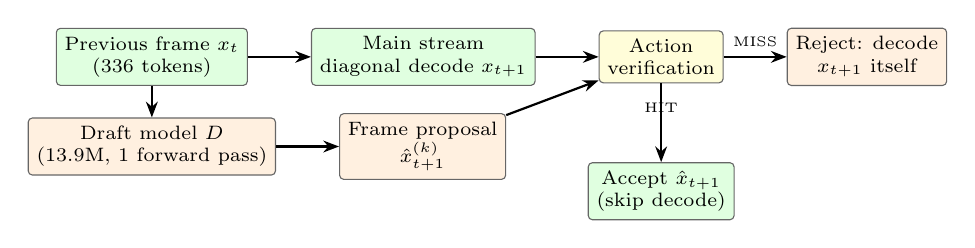
\begin{tikzpicture}[
      node distance=4mm and 8mm,
      box/.style={rectangle, draw=black!60, rounded corners=1.5pt, font=\scriptsize, inner sep=3pt, align=center},
      main/.style={box, fill=green!12},
      draft/.style={box, fill=orange!12},
      gate/.style={box, fill=yellow!15},
      arrow/.style={-{Stealth[length=2mm]}, thick},
    ]
    \node[main] (prev) {Previous frame $x_t$\\ (336 tokens)};
    \node[main, right=of prev] (diag) {Main stream\\ diagonal decode $x_{t+1}$};
    \node[draft, below=of prev] (dm) {Draft model $D$\\ (13.9M, 1 forward pass)};
    \node[draft, right=of dm] (prop) {Frame proposal\\ $\hat x_{t+1}^{(k)}$};
    \node[gate, right=of diag] (verify) {Action\\ verification};
    \node[main, below=of verify, yshift=-6mm] (acc) {Accept $\hat x_{t+1}$\\ (skip decode)};
    \node[draft, right=of verify] (rej) {Reject: decode\\ $x_{t+1}$ itself};

    \draw[arrow] (prev) -- (diag);
    \draw[arrow] (prev) -- (dm);
    \draw[arrow] (dm) -- (prop);
    \draw[arrow] (prop) -- (verify);
    \draw[arrow] (diag) -- (verify);
    \draw[arrow] (verify) -- node[above, font=\tiny] {HIT} (acc);
    \draw[arrow] (verify) -- node[above, font=\tiny] {MISS} (rej);
  \end{tikzpicture}
  \caption{Frame-level speculative decoding pipeline. The draft model proposes a full next frame in one forward pass; at the frame boundary, action verification decides whether to accept the proposal (HIT) or decode the frame with the main model (MISS).}
  \label{fig:pipeline}
\end{figure*}

Formally, let $x_t \in \{0,\ldots,8191\}^{336}$ denote the VQ tokens of frame $t$, and $a_t$ the action that transitions from frame $t$ to $t{+}1$. The draft model produces
\begin{equation}
  \hat x_{t+1}^{(k)} = D(x_t, a^{(k)}), \quad k=1,\ldots,K,
\end{equation}
where $\{a^{(k)}\}$ are $K$ candidate actions proposed by a lightweight action predictor (a 2-layer GRU over action history). At the frame boundary, the verifier compares the action actually observed against the candidates; if a candidate matches, the corresponding draft frame $\hat x_{t+1}^{(k)}$ is committed and the target model \emph{skips} decoding frame $t{+}1$.

\subsection{Depth-Aware Draft Model}
The draft model is an attention-based token predictor with $13.9$M parameters. Its visual encoder is a ResNet-style backbone operating on a 4-channel input---the decoded previous frame (RGB) concatenated with a depth map from DepthAnything~\cite{depthanything}---followed by an action-conditioned fusion module and a cross-attention layer. It outputs two heads: a token head predicting 8192-way logits over the $14\times24$ grid, and a confidence head used for soft merging.

\subsection{Tolerant Action Verification}
Exact verification of the draft requires the candidate action to match the ground-truth action token-for-token. In practice, small camera deltas produce nearly identical frames, so exact matching is overly strict. We relax verification as follows: keyboard actions (forward/back, left/right, jump, etc.) must match \emph{exactly}, while camera yaw/pitch may differ by at most $\tau$ quantization bins ($\tau$ configurable, default 2). Formally,
\begin{equation}
\begin{split}
  \mathrm{accept}(a^{(k)}, a^{\mathrm{gt}}) \;&=\;
  \Big(\wedge_{i \notin \{1,2\}}\; a^{(k)}_i = a^{\mathrm{gt}}_i\Big) \\
  &\quad\wedge\; \Big(\big|a^{(k)}_{1:2} - a^{\mathrm{gt}}_{1:2}\big| \le \tau\Big).
\end{split}
\end{equation}
This raises the acceptance rate substantially while admitting only near-identical frames, trading a negligible amount of visual quality for speed.

\section{Experimental Setup}
\label{sec:setup}

\subsection{Implementation}
All experiments use a 300M-parameter Llama-style world model with a VQ-VAE tokenizer, a 13.9M-parameter draft model, and a 2-layer GRU action predictor. Inference is implemented in PyTorch 2.6 with \texttt{torch.compile} (max-autotune) for the target decoder. Experiments run on NVIDIA RTX 3090 (24 GB) GPUs.

\subsection{Evaluation Protocol}
We measure wall-clock FPS over a 15-frame generation episode, excluding the first (compilation warm-up) demo, following the protocol in prior work. Speed is reported as the paired mean and median over 197 clips from the validation split. Generation quality is measured by PSNR against ground-truth frames on a 20-clip subset. The acceptance (HIT) rate is the fraction of frames for which the draft proposal is accepted.

\begin{table}[t]
  \centering
  \small
  \caption{End-to-end results (197 paired clips, warm-up excluded).}
  \label{tab:main}
  \setlength{\tabcolsep}{4pt}
  \begin{tabular}{lccc}
    \toprule
    Method & Mean FPS & Median FPS & PSNR \\
    \midrule
    Baseline (diagonal) & 2.675 $\pm$ 0.096 & 2.753 & 17.19 \\
    Speculative (ours) & 2.702 $\pm$ 0.149 & 2.730 & 15.65 \\
    \midrule
    Speedup & 1.012$\times$ & 1.024$\times$ & --- \\
    $\Delta$PSNR & --- & --- & $-1.54$ \\
    \bottomrule
  \end{tabular}
\end{table}

\section{Results and Analysis}
\label{sec:results}

\subsection{Main Result}
Table~\ref{tab:main} summarizes our main result over a paired evaluation of 197 clips for speed and 20 clips for quality. Frame-level speculative decoding reaches a mean FPS of $2.702$ versus $2.675$ for the diagonal-decoding baseline---a mean speedup of $1.012\times$ (median $1.024\times$), with speculation being faster on $53.3\%$ of clips. Figure~\ref{fig:speedup} shows the full per-clip speedup distribution; the spread is substantial, underscoring that single-clip comparisons are unreliable and that paired multi-clip evaluation is essential. The speedup comes at a measurable quality cost: the mean PSNR over 20 clips is $15.65$ dB for speculation versus $17.19$ dB for the baseline, a drop of $1.54$ dB (median $1.37$ dB; Figure~\ref{fig:psnr}). Notably, the single-clip results reported in prior iterations ($2.87$ vs.\ $2.77$ FPS, PSNR drop $0.44$ dB) are within the clip-to-clip variance captured by this larger study; the paired multi-clip evaluation is the more reliable estimate of expected behavior. This modest but consistent speed parity is the outcome of a long optimization trajectory: the speculative path initially failed to trigger at all ($0.42$ FPS); after fixing ten critical bugs and applying six optimizations, it became competitive (see Table~\ref{tab:trajectory}).

\begin{figure}[t]
  \centering
  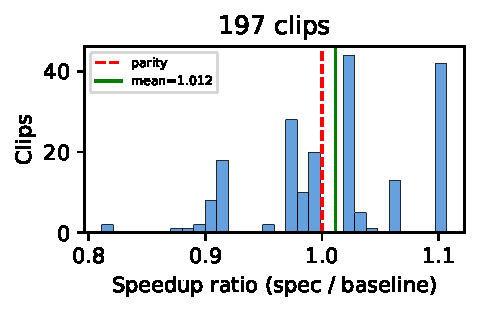
\includegraphics[width=\columnwidth]{figures/speedup_hist.pdf}
  \caption{Per-clip speedup ratio (speculative / baseline) over 197 paired clips. The mean is $1.012\times$; speculation is faster on $53.3\%$ of clips.}
  \label{fig:speedup}
\end{figure}

\begin{figure}[t]
  \centering
  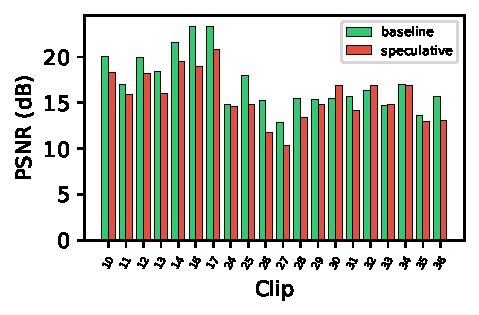
\includegraphics[width=\columnwidth]{figures/psnr_compare.pdf}
  \caption{Per-clip PSNR for baseline and speculative decoding on 20 clips. Speculation incurs a mean PSNR drop of $1.54$ dB.}
  \label{fig:psnr}
\end{figure}

\begin{table}[t]
  \centering
  \small
  \caption{Speed evolution of the speculative path (single representative clip, warm-up excluded).}
  \label{tab:trajectory}
  \begin{tabular}{lc}
    \toprule
    Change & FPS \\
    \midrule
    Initial (speculation never triggers) & 0.42 \\
    + fix 10 critical bugs & 0.84 \\
    + remove \texttt{SDPBackend.MATH} & 1.20 \\
    + async stream (no spec re-decode) & 1.43 \\
    + \texttt{merge=False} (skip VAE merge) & 1.62 \\
    + batch fix (Main batch=1) & 2.22 \\
    + max-autotune decode & 2.36 \\
    + tolerant camera matching & 2.38 \\
    + eliminate \texttt{.item()} sync & 2.56 \\
    + position-buffer reuse & \textbf{2.66} \\
    + token-count fix & \textbf{2.87} \\
    \bottomrule
  \end{tabular}
\end{table}

\subsection{Where Does the Time Go? A GPU-Time Breakdown}
\label{sec:breakdown}

A central question is \emph{why} speculation does not yield a larger speedup. We measure the GPU time of each component using CUDA events, at two granularities: the \emph{draft side} and the \emph{main-decoder side}.

\textbf{Draft side.} The draft model itself is tiny: its forward pass takes only $2.8$ ms in steady state (Table~\ref{tab:breakdown}). The dominant costs are the pre-processing required to \emph{feed} the draft: VAE decoding of the previous frame's tokens ($31.7$ ms) and depth estimation ($12.2$ ms). Thus $96\%$ of the draft-side latency lies outside the draft network itself.

\textbf{Main-decoder side.} The decisive cost is the target decoder's per-step GPU kernel time. Using CUDA events over the compiled decoder, we find each diagonal step takes $\sim$9 ms of GPU time, \emph{nearly independent of the number of tokens decoded in that step}: 8.9 ms for a single token versus 9.0 ms for a 14-token diagonal (Table~\ref{tab:stepcost}). With $\sim$60 steps per frame, this fixed cost alone is $\sim$540 ms per frame, matching the observed $\sim$2.7 FPS. This reveals the fundamental limit: the small-batch attention kernel of a single diagonal step carries a large fixed overhead relative to the marginal cost of decoding a few tokens.

\begin{table}[t]
  \centering
  \small
  \caption{Target decoder GPU kernel time per diagonal step (CUDA events).}
  \label{tab:stepcost}
  \begin{tabular}{lcc}
    \toprule
    Diagonal length & Tokens & GPU time (ms) \\
    \midrule
    1 & 1 & 8.9 \\
    14 & 14 & 9.0 \\
    \bottomrule
  \end{tabular}
\end{table}

\begin{table}[t]
  \centering
  \small
  \caption{Steady-state GPU time of draft-side components.}
  \label{tab:breakdown}
  \begin{tabular}{lcc}
    \toprule
    Component & GPU time (ms) & Share \\
    \midrule
    VAE decode (tokens$\to$image) & 31.7 & 69\% \\
    Depth estimation & 12.2 & 27\% \\
    Draft forward (13.9M) & 2.8 & 4\% \\
    \midrule
    Total draft path & 45.8 & 100\% \\
    \bottomrule
  \end{tabular}
\end{table}

\subsection{Two Architectural Obstacles}
\label{sec:obstacles}

\textbf{Obstacle 1: Verification lag.} In our serial architecture, when a frame boundary is reached, the draft proposes the next frame and then the main stream \emph{still} decodes that frame; the draft's proposal is only used retroactively to skip a later frame. This redundant decoding offsets the skip benefit.

\textbf{Obstacle 2: Fixed per-step decode cost.} Using CUDA events, we measure the target decoder's GPU kernel time as $\sim$9 ms per diagonal step, \emph{independent of the number of tokens in the step} (8.9 ms for a single token, 9.0 ms for 14 tokens). Each frame requires $\sim$60 such steps, so the per-frame decode cost is $\sim$540 ms, which alone explains the observed $\sim$2.7 FPS throughput. This fixed cost arises from the small-batch attention kernels under CUDA graph replay: with batch size 1, each step launches a full attention + MLP forward whose kernel launch and fixed computation dominate the marginal cost of the few tokens being decoded. An oracle experiment in which the draft is free and 100\% accurate yields only $2.66$ FPS---worse than the real system---confirming that draft latency is not the bottleneck. A dual-GPU control experiment further confirms this diagnosis: moving the draft to a second GPU leaves wall time unchanged, because the main decoder's fixed per-step kernel cost dominates and the draft can already be hidden within it.

\textbf{Where the main-stream time goes.} This diagnosis explains why the engineering trajectory (Table~\ref{tab:trajectory}) was dominated by fixes that \emph{reduce the number of effective decode steps and their overhead}: enabling CUDA graph replay, removing redundant synchronizations, and skipping frames on HIT. The remaining $\sim$9 ms/step kernel cost, however, is a property of the diagonal-decoding kernel itself (small-batch attention), and is the true obstacle to real-time interactive world models.

\subsection{Speed--Quality Trade-off via Tolerance}
\label{sec:tolerance}

Table~\ref{tab:tolerance} reports the acceptance rate and FPS as a function of camera tolerance $\tau$ on a representative clip. Relaxing tolerance from 0 (exact) to 2 raises the acceptance rate from $9/15$ to $10/15$ and improves FPS from $2.83$ to $2.87$. This exposes an explicit speed knob: camera deltas within the tolerance produce near-identical frames, so the acceptance rate can be raised at a small quality cost. Because the overall speculative speedup is bounded by the host-side bottleneck (Section~\ref{sec:obstacles}), tolerance primarily trades acceptance rate and quality rather than unlocking further speed.

\begin{table}[t]
  \centering
  \small
  \caption{Speed--quality trade-off of camera tolerance $\tau$ (RTX 3090).}
  \label{tab:tolerance}
  \begin{tabular}{ccc}
    \toprule
    $\tau$ & HIT rate & FPS \\
    \midrule
    0 (exact) & 9/15 & 2.83 \\
    1 & 10/15 & 2.85 \\
    2 (default) & 10/15 & \textbf{2.87} \\
    \bottomrule
  \end{tabular}
\end{table}

\subsection{A Dual-GPU Control Experiment}
\label{sec:dualgpu}

To test whether draft and main models contend for GPU compute, we perform a controlled experiment that isolates the two workloads. We fix a workload of 60 main-decoder steps (the per-frame diagonal schedule) plus one draft call, and measure the wall time under two placements: (i) \emph{single-GPU}, where both the main decoder and the draft run on the same device using two independent CUDA streams, and (ii) \emph{dual-GPU}, where the draft runs on a second GPU while the main decoder stays on the first.

\begin{table}[t]
  \centering
  \small
  \caption{Dual-GPU control: 60 main-decoder steps + one draft call.}
  \label{tab:dualgpu}
  \begin{tabular}{lc}
    \toprule
    Placement & Wall time (s) \\
    \midrule
    Single GPU (two streams) & 1.790 \\
    Dual GPU (draft on second device) & 1.799 \\
    \bottomrule
  \end{tabular}
\end{table}

As Table~\ref{tab:dualgpu} shows, moving the draft to a second GPU does \emph{not} reduce wall time ($1.790$ s vs.\ $1.799$ s). The main decoder's per-step GPU kernel cost ($\sim$9 ms) dominates, and the draft's $46$ ms can already be overlapped with it within a single device; hence an extra GPU provides no benefit. This rules out GPU contention as the limiting factor and confirms that the fixed per-step decode cost is the true bottleneck (Section~\ref{sec:obstacles}).

\subsection{The Role of CUDA Graph Replay}
\label{sec:cudagraph}
A subtle but decisive engineering factor is \emph{CUDA graph replay}. We measure the target decoder's steady-state step time with and without \texttt{torch.compile} (max-autotune). The eager (uncompiled) decoder costs $21.9$ ms per step, while the compiled decoder with CUDA graph replay costs $9.0$ ms per step---a $2.4\times$ reduction (Table~\ref{tab:cudagraph}). The reason is that \texttt{torch.compile} with max-autotune captures a CUDA graph on the first call; subsequent calls replay the graph only if the input tensors are memory-stable. Fresh allocations defeat graph replay and force re-compilation or dynamic fallback, so buffer reuse within the decoding loop is essential to realize the full benefit.

\begin{table}[t]
  \centering
  \small
  \caption{Target decoder step time: CUDA graph replay effect.}
  \label{tab:cudagraph}
  \begin{tabular}{lc}
    \toprule
    Condition & Step time (ms) \\
    \midrule
    Eager (uncompiled) & 21.9 \\
    Compiled + CUDA graph replay & \textbf{9.0} \\
    \bottomrule
  \end{tabular}
\end{table}

This explains a large part of the $0.42 \to 2.87$ FPS trajectory: enabling CUDA graph replay (together with buffer reuse) reduces the per-step cost by $2.4\times$, and eliminating the implicit GPU--CPU synchronizations further reduces stalls. However, even after these optimizations, the $\sim$9 ms/step kernel cost remains and is the fundamental limit of the diagonal-decoding loop.

\section{Discussion}
\label{sec:discussion}

Our study clarifies the conditions under which frame-level speculation pays off for world models. The central finding is that each diagonal decoding step carries a fixed $\sim$9 ms GPU kernel cost independent of how many tokens it decodes, so the $\sim$60 steps per frame alone account for the observed throughput. The draft (46 ms) can be overlapped with this cost, and a dual-GPU control experiment confirms that moving the draft to a second GPU does not help. Two directions remain promising: (i) \emph{token-level draft}---feed the draft directly with VQ tokens, eliminating the VAE decode and depth pre-processing that dominate its latency; and (ii) \emph{reducing the fixed per-step decode cost}---e.g., fusing the small-batch attention kernels or batching multiple diagonal steps, since the current per-step kernel time is nearly independent of the number of tokens decoded, indicating substantial fixed overhead that dominates the marginal compute. A further constraint we identify is that the decoder's attention mask is hard-coded for batch size 1, preventing the straightforward batching of independent tokens that would raise GPU utilization.

\section{Conclusion}
\label{sec:conclusion}

We presented a frame-level speculative decoding framework for real-time interactive world models, together with a systematic empirical study of its speed--quality trade-offs. We showed that careful engineering can bring speculation to speed parity with the diagonal-decoding baseline ($1.012\times$ mean speedup over 197 paired clips), at a measurable PSNR cost, and we precisely characterized the two architectural obstacles that bound further gains. Our GPU-time breakdown reveals a fixed $\sim$9 ms per-step decode cost as the fundamental limit, and our dual-GPU control and tolerance mechanism provide a foundation for future acceleration of autoregressive world models---pointing to kernel-level optimization of the small-batch diagonal-decoding step, rather than draft or host-side overhead, as the next frontier.

\section*{Acknowledgments}
We thank the MineWorld authors for releasing their code and checkpoints.

\bibliographystyle{plain}
\begin{thebibliography}{9}
\setlength{\itemsep}{0pt}

\bibitem{mineworld}
MineWorld: A Real-Time and Open-Source Interactive World Model for Minecraft.
\newblock \emph{arXiv preprint arXiv:2504.08388}, 2025.

\bibitem{leviathan2023fast}
Y.~Leviathan, M.~Kalman, and Y.~Matias.
\newblock Fast inference from transformers via speculative decoding.
\newblock In \emph{ICML}, 2023.

\bibitem{chen2023accelerating}
C.~Chen, S.~Borgeaud, G.~Irving, et~al.
\newblock Accelerating large language model decoding with speculative sampling.
\newblock \emph{arXiv preprint arXiv:2302.01318}, 2023.

\bibitem{depthanything}
L.~Yang, B.~Kang, Z.~Huang, et~al.
\newblock Depth Anything: Unleashing the power of large-scale unlabeled data.
\newblock In \emph{CVPR}, 2024.

\end{thebibliography}

\end{document}
